% ============================================================
%  Příprava na maturitu – Elektrotechnika
%  Okruh 2: Elektrostatické pole
% ============================================================

\documentclass[a4paper,10pt]{article}

\usepackage[T1]{fontenc}
\usepackage[utf8]{inputenc}
\usepackage[left=2.0cm, right=1.8cm, top=1.8cm, bottom=1.8cm]{geometry}
\usepackage{parskip}
\usepackage{xcolor}
\usepackage{tabularx}
\usepackage{booktabs}
\usepackage{tikz}
\usepackage{mdframed}
\usepackage{amsmath}
\usepackage{enumitem}
\usepackage{circuitikz}

\usetikzlibrary{arrows.meta, positioning, decorations.pathmorphing, shapes.geometric}

% --- Barvy ---
\definecolor{accent}{HTML}{1A3A5C}
\definecolor{lightblue}{HTML}{EAF2F8}
\definecolor{lightyellow}{HTML}{FDFBE4}
\definecolor{lightgreen}{HTML}{EAF7EA}
\definecolor{lightred}{HTML}{FDE8E8}
\definecolor{lightgray}{HTML}{F4F4F4}

% --- Boxy ---
\newmdenv[backgroundcolor=lightblue,linecolor=accent!40,roundcorner=4pt,
  innertopmargin=6pt,innerbottommargin=6pt,innerleftmargin=8pt,innerrightmargin=8pt]{pojmybox}
\newmdenv[backgroundcolor=lightyellow,linecolor=accent!30,roundcorner=4pt,
  innertopmargin=6pt,innerbottommargin=6pt,innerleftmargin=8pt,innerrightmargin=8pt]{vysvetlenibox}
\newmdenv[backgroundcolor=lightgreen,linecolor=accent!40,roundcorner=4pt,
  innertopmargin=6pt,innerbottommargin=6pt,innerleftmargin=8pt,innerrightmargin=8pt]{vzorcebox}
\newmdenv[backgroundcolor=lightred,linecolor=accent!30,roundcorner=4pt,
  innertopmargin=6pt,innerbottommargin=6pt,innerleftmargin=8pt,innerrightmargin=8pt]{durazbox}

\setlist[itemize]{noitemsep, leftmargin=1.4em, topsep=2pt}
\setlist[enumerate]{noitemsep, leftmargin=1.4em, topsep=2pt}

% --- Zkratka pro jednotky ---
\newcommand{\jednotka}[1]{\,[\mathrm{#1}]}

\begin{document}

% ============================================================
\section*{\large Okruh 2 – Elektrostatické pole}

\begin{pojmybox}
\textbf{Klíčové pojmy:}
elektrický náboj, Coulombův zákon, intenzita elektrického pole, siločáry, elektrický potenciál, elektrické napětí, kapacita, kondenzátor, permitivita, polarizace dielektrika, elektrostatická indukce
\end{pojmybox}

\begin{vysvetlenibox}

% ================================================================
\subsection*{1. Elektrický náboj a Coulombův zákon}

\textbf{Elektrický náboj} $Q$ je fyzikální veličina vyjadřující schopnost tělesa působit elektrickou silou. Existuje kladný (protony) a záporný (elektrony). Elementární náboj je $e \approx 1{,}602 \cdot 10^{-19}\mathrm{C}$. 

Souhlasné náboje se odpuzují, nesouhlasné se přitahují. Velikost této síly popisuje \textbf{Coulombův zákon}.

\begin{vzorcebox}
\[
F_e = \frac{1}{4\pi\varepsilon} \cdot \frac{|Q_1 \cdot Q_2|}{r^2} \jednotka{N}
\]
kde $F_e$ = elektrická síla [N], $Q_1, Q_2$ = bodové náboje [C], $r$ = vzdálenost nábojů [m], $\varepsilon$ = permitivita prostředí [F/m].
\end{vzorcebox}

\begin{center}
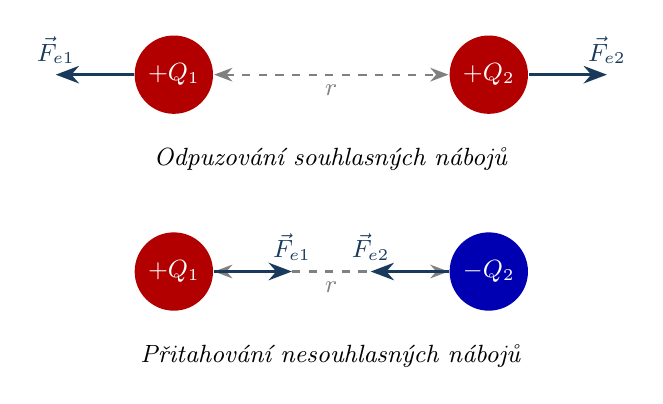
\begin{tikzpicture}[>=Stealth, font=\small, thick]
  % Odpuzování (souhlasné)
  \node[circle, fill=red!70!black, text=white, inner sep=3pt] (q1) at (0,0) {$+Q_1$};
  \node[circle, fill=red!70!black, text=white, inner sep=3pt] (q2) at (4,0) {$+Q_2$};
  \draw[<->, dashed, gray] (q1) -- (q2) node[midway, below] {$r$};
  \draw[->, accent, line width=1.2pt] (q1) -- (-1.5,0) node[above] {$\vec{F}_{e1}$};
  \draw[->, accent, line width=1.2pt] (q2) -- (5.5,0) node[above] {$\vec{F}_{e2}$};
  \node[below=0.8cm] at (2,0) {\textit{Odpuzování souhlasných nábojů}};

  % Přitahování (nesouhlasné)
  \begin{scope}[yshift=-2.5cm]
    \node[circle, fill=red!70!black, text=white, inner sep=3pt] (q3) at (0,0) {$+Q_1$};
    \node[circle, fill=blue!70!black, text=white, inner sep=3pt] (q4) at (4,0) {$-Q_2$};
    \draw[<->, dashed, gray] (q3) -- (q4) node[midway, below] {$r$};
    \draw[->, accent, line width=1.2pt] (q3) -- (1.5,0) node[above] {$\vec{F}_{e1}$};
    \draw[->, accent, line width=1.2pt] (q4) -- (2.5,0) node[above] {$\vec{F}_{e2}$};
    \node[below=0.8cm] at (2,0) {\textit{Přitahování nesouhlasných nábojů}};
  \end{scope}
\end{tikzpicture}
\end{center}

Permitivita prostředí $\varepsilon = \varepsilon_0 \cdot \varepsilon_r$, kde $\varepsilon_0 \approx 8{,}85 \cdot 10^{-12}\,\mathrm{F/m}$ (permitivita vakua) a $\varepsilon_r$ je relativní permitivita (pro vakuum/vzduch $\varepsilon_r \approx 1$).

% ================================================================
\subsection*{2. Elektrické pole a siločáry}

Kolem každého elektrického náboje existuje elektrické pole. Jeho silové účinky popisuje \textbf{intenzita elektrického pole} $\vec{E}$. Je to vektorová veličina určující sílu, která působí na jednotkový kladný zkušební náboj.

\begin{vzorcebox}
\[
E = \frac{F_e}{q} \jednotka{V/m} \text{ nebo } \jednotka{N/C}
\qquad
\text{Pro bodový náboj:} \quad E = \frac{1}{4\pi\varepsilon} \cdot \frac{Q}{r^2}
\]
\end{vzorcebox}

Graficky se pole znázorňuje \textbf{siločárami}. Ty vždy vystupují z kladného náboje a vstupují do záporného.

\begin{center}
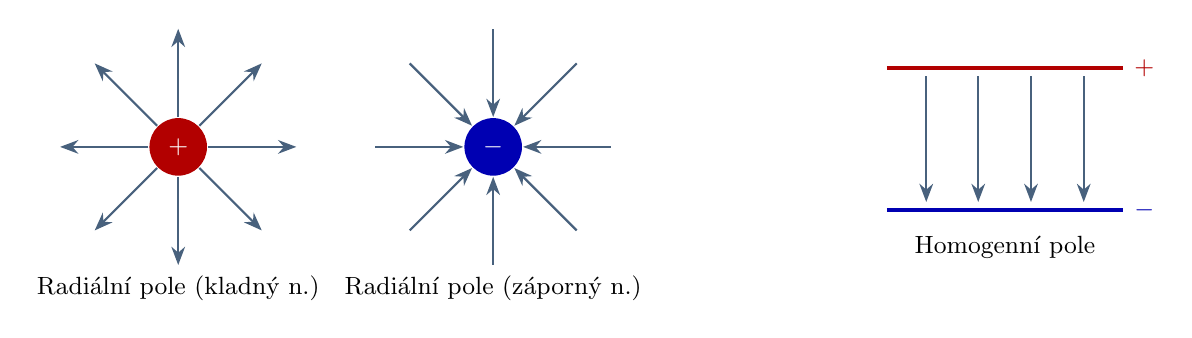
\begin{tikzpicture}[>=Stealth, font=\small, thick]
  % Radiální pole +
  \begin{scope}[xshift=0cm]
    \node[circle, fill=red!70!black, text=white, inner sep=4pt] (pos) at (0,0) {$+$};
    \foreach \angle in {0, 45, 90, 135, 180, 225, 270, 315} {
      \draw[->, accent!80] (pos) -- (\angle:1.5);
    }
    \node[below=1.5cm] at (0,0) {Radiální pole (kladný n.)};
  \end{scope}

  % Radiální pole -
  \begin{scope}[xshift=4cm]
    \node[circle, fill=blue!70!black, text=white, inner sep=4pt] (neg) at (0,0) {$-$};
    \foreach \angle in {0, 45, 90, 135, 180, 225, 270, 315} {
      \draw[<-, accent!80] (neg) -- (\angle:1.5);
    }
    \node[below=1.5cm] at (0,0) {Radiální pole (záporný n.)};
  \end{scope}

  % Homogenní pole
  \begin{scope}[xshift=9cm, yshift=-0.8cm]
    \draw[line width=1.5pt, red!70!black] (0,1.8) -- (3,1.8) node[right] {$+$};
    \draw[line width=1.5pt, blue!70!black] (0,0) -- (3,0) node[right] {$-$};
    \foreach \x in {0.5, 1.16, 1.83, 2.5} {
      \draw[->, accent!80] (\x, 1.7) -- (\x, 0.1);
    }
    \node[below=0.2cm] at (1.5,0) {Homogenní pole};
  \end{scope}
\end{tikzpicture}
\end{center}

% ================================================================
\subsection*{3. Práce, potenciál a napětí v elektrickém poli}

\textbf{Práce ($W$):} Při přemísťování náboje v elektrickém poli se koná práce. Nezávisí na tvaru trajektorie, ale pouze na počátečním a koncovém bodě.
\textbf{Elektrický potenciál ($\varphi$):} Potenciální energie jednotkového náboje v daném bodě pole.
\textbf{Elektrické napětí ($U$):} Rozdíl potenciálů mezi dvěma body.

\begin{vzorcebox}
\[
\varphi = \frac{W}{Q} \jednotka{V}
\qquad
U = \varphi_1 - \varphi_2 = \frac{W}{Q} \jednotka{V}
\qquad
\text{V homogenním poli:} \quad E = \frac{U}{d}
\]
kde $d$ je vzdálenost mezi deskami (body) ve směru siločar.
\end{vzorcebox}

% ================================================================
\subsection*{4. Kapacita a kondenzátor}

\textbf{Kapacita ($C$)} vyjadřuje schopnost vodiče (nebo soustavy vodičů) pojmout elektrický náboj při určitém napětí. Součástka konstruovaná pro uchování náboje se nazývá \textbf{kondenzátor} (většinou dvě vodivé desky oddělené dielektrikem).

\begin{vzorcebox}
\[
C = \frac{Q}{U} \jednotka{F} \quad \text{(farad)}
\qquad
\text{Deskový kondenzátor:} \quad C = \varepsilon_0 \cdot \varepsilon_r \cdot \frac{S}{d}
\]
kde $S$ = účinná plocha desek [m$^2$], $d$ = vzdálenost desek [m], $\varepsilon_r$ = relativní permitivita dielektrika.
\end{vzorcebox}

\begin{center}
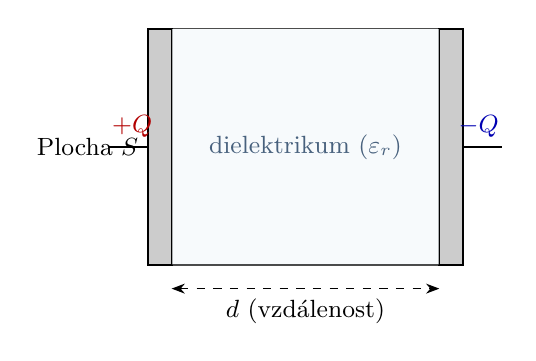
\begin{tikzpicture}[>=Stealth, font=\small]
  % Desky
  \draw[thick, fill=gray!40] (0,0) rectangle (0.3,3);
  \draw[thick, fill=gray!40] (3.7,0) rectangle (4.0,3);
  
  % Dielektrikum
  \draw[fill=lightblue!50, opacity=0.7] (0.3,0) rectangle (3.7,3);
  \node[text=accent!80] at (2,1.5) {dielektrikum ($\varepsilon_r$)};

  % Popisy
  \draw[<->, dashed] (0.3, -0.3) -- (3.7, -0.3) node[midway, below] {$d$ (vzdálenost)};
  \node[left] at (0, 1.5) {Plocha $S$};
  
  % Připojení
  \draw[thick] (-0.5, 1.5) -- (0, 1.5);
  \draw[thick] (4.0, 1.5) -- (4.5, 1.5);
  \node[above, text=red!70!black] at (-0.2, 1.5) {$+Q$};
  \node[above, text=blue!70!black] at (4.2, 1.5) {$-Q$};
\end{tikzpicture}
\end{center}

% ================================================================
\subsection*{5. Spojování kondenzátorů}

\begin{durazbox}
\textbf{Pozor!} Vzorce pro spojování kondenzátorů jsou přesně \textbf{opačné} než u rezistorů.
\end{durazbox}

\subsubsection*{Paralelní zapojení (vedle sebe)}

\begin{center}
\begin{circuitikz}[font=\small]
  \draw (0,1.5)
    to[short, o-] (1,1.5)
    to[short] (1,2.5)
    to[C, l=$C_1$] (4,2.5)
    to[short] (4,1.5);
  \draw (1,1.5)
    to[C, l=$C_2$] (4,1.5);
  \draw (1,1.5)
    to[short] (1,0.5)
    to[C, l=$C_3$] (4,0.5)
    to[short] (4,1.5)
    to[short, -o] (5,1.5);
  \node[left] at (0,1.5) {$U$};
\end{circuitikz}
\end{center}

\begin{vzorcebox}
\[
C_{celk} = C_1 + C_2 + C_3 + \cdots
\qquad
Q_{celk} = Q_1 + Q_2 + Q_3
\qquad
U = \text{const.}
\]
\end{vzorcebox}
\textit{Zvětšuje se celková účinná plocha desek $\rightarrow$ kapacita roste.}

\subsubsection*{Sériové zapojení (za sebou)}

\begin{center}
\begin{circuitikz}[font=\small]
  \draw (0,0)
    to[short, o-] (0.5,0)
    to[C, l=$C_1$] (2.5,0)
    to[C, l=$C_2$] (4.5,0)
    to[C, l=$C_3$] (6.5,0)
    to[short, -o] (7,0);
  \node[below] at (0,0) {$U$};
  \draw[->, thick, accent] (0.2,-0.6) -- (6.8,-0.6) node[midway, below] {$Q$ – stejný náboj všude};
\end{circuitikz}
\end{center}

\begin{vzorcebox}
\[
\frac{1}{C_{celk}} = \frac{1}{C_1} + \frac{1}{C_2} + \frac{1}{C_3}
\qquad
\text{(pro 2 kondenzátory: } C_{celk} = \frac{C_1 \cdot C_2}{C_1 + C_2} \text{)}
\]
\[
U_{celk} = U_1 + U_2 + U_3
\qquad
Q = \text{const.}
\]
\end{vzorcebox}
\textit{Zvětšuje se celková vzdálenost desek $\rightarrow$ kapacita klesá. Slouží k rozložení vysokého napětí.}

% ================================================================
\subsection*{6. Chování látek v elektrickém poli}

\textbf{Vodiče (Elektrostatická indukce):} Vložíme-li do elektrického pole nenabitý vodič, volné elektrony se přesunou proti směru siločar. Na jedné straně vznikne přebytek elektronů ($-$) a na druhé jejich nedostatek ($+$). Uvnitř vodiče je výsledná intenzita pole nulová.

\textbf{Izolanty/Dielektrika (Polarizace):} Izolanty nemají volné elektrony. Vložením do pole dojde k deformaci elektronových obalů atomů (nebo natočení polárních molekul). Na povrchu dielektrika se objeví vázané polarizační náboje, které zeslabují vnější elektrické pole uvnitř látky (proto platí $\varepsilon_r > 1$).

% ================================================================
\subsection*{7. Energie nabitého kondenzátoru}

Při nabíjení kondenzátoru se koná práce, která se uchovává ve formě energie elektrického pole.
\begin{vzorcebox}
\[
W = \frac{1}{2} \cdot C \cdot U^2 = \frac{1}{2} \cdot Q \cdot U = \frac{1}{2} \cdot \frac{Q^2}{C} \jednotka{J}
\]
\end{vzorcebox}

% ================================================================
\subsection*{8. Shrnutí – přehled vzorců}

\begin{center}
\begin{tabularx}{0.97\linewidth}{@{} l l l @{}}
\toprule
\textbf{Veličina} & \textbf{Vzorec} & \textbf{Jednotka} \\
\midrule
Coulombův zákon & $F_e = \dfrac{1}{4\pi\varepsilon_0\varepsilon_r} \cdot \dfrac{|Q_1 Q_2|}{r^2}$ & N (newton) \\
Intenzita el. pole & $E = F_e / q = U / d$ & V/m (nebo N/C) \\
Potenciál / Napětí & $\varphi = W / Q \quad U = \varphi_1 - \varphi_2$ & V (volt) \\
Kapacita & $C = Q / U$ & F (farad) \\
Deskový kondenzátor & $C = \varepsilon_0 \cdot \varepsilon_r \cdot S / d$ & F \\
Energie kondenzátoru & $W = \dfrac{1}{2} \cdot C \cdot U^2$ & J (joule) \\
Sériové spojení $C$ & $1/C_{celk} = 1/C_1 + 1/C_2 + \cdots$ & F \\
Paralelní spojení $C$ & $C_{celk} = C_1 + C_2 + \cdots$ & F \\
\bottomrule
\end{tabularx}
\end{center}

\end{vysvetlenibox}

\end{document}